% Options for packages loaded elsewhere
\PassOptionsToPackage{unicode}{hyperref}
\PassOptionsToPackage{hyphens}{url}
%
\documentclass[
  american,
  man,floatsintext]{apa7}
\usepackage{lmodern}
\usepackage{amssymb,amsmath}
\usepackage{ifxetex,ifluatex}
\ifnum 0\ifxetex 1\fi\ifluatex 1\fi=0 % if pdftex
  \usepackage[T1]{fontenc}
  \usepackage[utf8]{inputenc}
  \usepackage{textcomp} % provide euro and other symbols
\else % if luatex or xetex
  \usepackage{unicode-math}
  \defaultfontfeatures{Scale=MatchLowercase}
  \defaultfontfeatures[\rmfamily]{Ligatures=TeX,Scale=1}
\fi
% Use upquote if available, for straight quotes in verbatim environments
\IfFileExists{upquote.sty}{\usepackage{upquote}}{}
\IfFileExists{microtype.sty}{% use microtype if available
  \usepackage[]{microtype}
  \UseMicrotypeSet[protrusion]{basicmath} % disable protrusion for tt fonts
}{}
\makeatletter
\@ifundefined{KOMAClassName}{% if non-KOMA class
  \IfFileExists{parskip.sty}{%
    \usepackage{parskip}
  }{% else
    \setlength{\parindent}{0pt}
    \setlength{\parskip}{6pt plus 2pt minus 1pt}}
}{% if KOMA class
  \KOMAoptions{parskip=half}}
\makeatother
\usepackage{xcolor}
\IfFileExists{xurl.sty}{\usepackage{xurl}}{} % add URL line breaks if available
\IfFileExists{bookmark.sty}{\usepackage{bookmark}}{\usepackage{hyperref}}
\hypersetup{
  pdftitle={Introduction},
  pdfauthor={Cillian McHugh1, Marek McGann2, Eric R. Igou1, \& Elaine L Kinsella1},
  pdflang={en-US},
  pdfkeywords={keywords},
  hidelinks,
  pdfcreator={LaTeX via pandoc}}
\urlstyle{same} % disable monospaced font for URLs
\usepackage{graphicx,grffile}
\makeatletter
\def\maxwidth{\ifdim\Gin@nat@width>\linewidth\linewidth\else\Gin@nat@width\fi}
\def\maxheight{\ifdim\Gin@nat@height>\textheight\textheight\else\Gin@nat@height\fi}
\makeatother
% Scale images if necessary, so that they will not overflow the page
% margins by default, and it is still possible to overwrite the defaults
% using explicit options in \includegraphics[width, height, ...]{}
\setkeys{Gin}{width=\maxwidth,height=\maxheight,keepaspectratio}
% Set default figure placement to htbp
\makeatletter
\def\fps@figure{htbp}
\makeatother
\setlength{\emergencystretch}{3em} % prevent overfull lines
\providecommand{\tightlist}{%
  \setlength{\itemsep}{0pt}\setlength{\parskip}{0pt}}
\setcounter{secnumdepth}{-\maxdimen} % remove section numbering
% Make \paragraph and \subparagraph free-standing
\ifx\paragraph\undefined\else
  \let\oldparagraph\paragraph
  \renewcommand{\paragraph}[1]{\oldparagraph{#1}\mbox{}}
\fi
\ifx\subparagraph\undefined\else
  \let\oldsubparagraph\subparagraph
  \renewcommand{\subparagraph}[1]{\oldsubparagraph{#1}\mbox{}}
\fi
% Manuscript styling
\usepackage{upgreek}
\captionsetup{font=singlespacing,justification=justified}

% Table formatting
\usepackage{longtable}
\usepackage{lscape}
% \usepackage[counterclockwise]{rotating}   % Landscape page setup for large tables
\usepackage{multirow}		% Table styling
\usepackage{tabularx}		% Control Column width
\usepackage[flushleft]{threeparttable}	% Allows for three part tables with a specified notes section
\usepackage{threeparttablex}            % Lets threeparttable work with longtable

% Create new environments so endfloat can handle them
% \newenvironment{ltable}
%   {\begin{landscape}\centering\begin{threeparttable}}
%   {\end{threeparttable}\end{landscape}}
\newenvironment{lltable}{\begin{landscape}\centering\begin{ThreePartTable}}{\end{ThreePartTable}\end{landscape}}

% Enables adjusting longtable caption width to table width
% Solution found at http://golatex.de/longtable-mit-caption-so-breit-wie-die-tabelle-t15767.html
\makeatletter
\newcommand\LastLTentrywidth{1em}
\newlength\longtablewidth
\setlength{\longtablewidth}{1in}
\newcommand{\getlongtablewidth}{\begingroup \ifcsname LT@\roman{LT@tables}\endcsname \global\longtablewidth=0pt \renewcommand{\LT@entry}[2]{\global\advance\longtablewidth by ##2\relax\gdef\LastLTentrywidth{##2}}\@nameuse{LT@\roman{LT@tables}} \fi \endgroup}

% \setlength{\parindent}{0.5in}
% \setlength{\parskip}{0pt plus 0pt minus 0pt}

% Overwrite redefinition of paragraph and subparagraph by the default LaTeX template
% See https://github.com/crsh/papaja/issues/292
\makeatletter
\renewcommand{\paragraph}{\@startsection{paragraph}{4}{\parindent}%
  {0\baselineskip \@plus 0.2ex \@minus 0.2ex}%
  {-1em}%
  {\normalfont\normalsize\bfseries\itshape\typesectitle}}

\renewcommand{\subparagraph}[1]{\@startsection{subparagraph}{5}{1em}%
  {0\baselineskip \@plus 0.2ex \@minus 0.2ex}%
  {-\z@\relax}%
  {\normalfont\normalsize\itshape\hspace{\parindent}{#1}\textit{\addperi}}{\relax}}
\makeatother

% \usepackage{etoolbox}
\makeatletter
\patchcmd{\HyOrg@maketitle}
  {\section{\normalfont\normalsize\abstractname}}
  {\section*{\normalfont\normalsize\abstractname}}
  {}{\typeout{Failed to patch abstract.}}
\patchcmd{\HyOrg@maketitle}
  {\section{\protect\normalfont{\@title}}}
  {\section*{\protect\normalfont{\@title}}}
  {}{\typeout{Failed to patch title.}}
\makeatother

\usepackage{xpatch}
\makeatletter
\xapptocmd\appendix
  {\xapptocmd\section
    {\addcontentsline{toc}{section}{\appendixname\ifoneappendix\else~\theappendix\fi\\: #1}}
    {}{\InnerPatchFailed}%
  }
{}{\PatchFailed}
\keywords{keywords\newline\indent Word count: TBC}
\usepackage{lineno}

\linenumbers
\usepackage{csquotes}
\usepackage[titles]{tocloft}
\cftpagenumbersoff{figure}
\renewcommand{\cftfigpresnum}{\itshape\figurename\enspace}
\renewcommand{\cftfigaftersnum}{.\space}
\setlength{\cftfigindent}{0pt}
\setlength{\cftafterloftitleskip}{0pt}
\settowidth{\cftfignumwidth}{Figure 10.\qquad}
\cftpagenumbersoff{table}
\renewcommand{\cfttabpresnum}{\itshape\tablename\enspace}
\renewcommand{\cfttabaftersnum}{.\space}
\setlength{\cfttabindent}{0pt}
\setlength{\cftafterloftitleskip}{0pt}
\settowidth{\cfttabnumwidth}{Table 10.\qquad}
\ifxetex
  % Load polyglossia as late as possible: uses bidi with RTL langages (e.g. Hebrew, Arabic)
  \usepackage{polyglossia}
  \setmainlanguage[variant=american]{english}
\else
  \usepackage[shorthands=off,main=american]{babel}
\fi

\title{Introduction}
\author{Cillian McHugh\textsuperscript{1}, Marek McGann\textsuperscript{2}, Eric R. Igou\textsuperscript{1}, \& Elaine L Kinsella\textsuperscript{1}}
\date{}


\shorttitle{Cognitive Load and Moral Dumbfounding}

\authornote{

Correspondence concerning this article should be addressed to Cillian McHugh, Mary Immaculate College, South Circular road, Limerick, Ireland. E-mail: \href{mailto:cillian.mchugh@ul.ie}{\nolinkurl{cillian.mchugh@ul.ie}}

}

\affiliation{\vspace{0.5cm}\textsuperscript{1} University of Limerick\\\textsuperscript{2} Mary Immaculate College \textasciitilde{} University of Limerick}

\abstract{%
Moral dumbfounding occurs when people defend a moral judgment even though they cannot provide a reason in support of this judgment. It manifests as an admission of not having reasons, or the use of unsupported declarations (\enquote{it’s just wrong}) or tautological reasons (\enquote{because it’s incest}) as justifications for a judgment. We test a dual-processes explanation of moral dumbfounding, where moral dumbfounding is an example of conflict between a habitual response (making a judgment) and a response that results from deliberation (providing a reason for the judgment). The dumbfounding paradigm involves three possible responses: (a) providing reasons for a judgment (deliberative/controlled process); (b) accepting the counter-arguments and rating the behaviour as \enquote{not wrong} (habitual/automatic process); (c) a dumbfounded response (habitual/automatic process). Cognitive load manipulations have been shown to inhibit deliberative responding. We present 6 studies in which dumbfounded responding was investigated under cognitive load manipulations. We hypothesized that rates of providing reasons would be reduced under cognitive load. The identification of reasons was inhibited in Studies 1, 2, 3, and 6, but not in Studies 4 or 5. The results provide some evidence for a dual-process explanation of moral dumbfounding. We found some evidence that dumbfounded responding may be linked with Need for Cognition.
}



\begin{document}
\maketitle

{
\setcounter{tocdepth}{3}
\tableofcontents
}
Moral dumbfounding occurs Moral dumbfounding occurs when people defend a moral judgment even though they cannot provide a reason in support of this judgment (Haidt et al., 2000; Haidt, 2001; see also McHugh, et al., 2017, 2020). It has traditionally been seen as evidence for intuitionist and dual-process theories of moral judgment (e.g., Crockett, 2013; Cushman, 2013; Cushman, Young, \& Greene, 2010; Greene, 2008; Haidt, 2001; Prinz, 2005; though this narrative has been contested, e.g., Guglielmo, 2018; Royzman, Kim, \& Leeman, 2015). Despite the influence of moral dumbfounding on the morality literature, the phenomenon is not well understood. In a pre-registered study we test one prediction of a conflict in dual-processes explanation of moral dumbfounding. By applying a cognitive load manipulation within a moral dumbfounding task we show that for three of the four moral scenarios used, dumbfounded responses are more likely when participants are engaged in a secondary task.

\hypertarget{moral-dumbfounding-a-dual-process-perspective}{%
\section{Moral Dumbfounding: A Dual-Process Perspective}\label{moral-dumbfounding-a-dual-process-perspective}}

Drawing on dual-process theories of moral judgment (e.g., Greene, 2008; Bago \& De Neys, 2019; Brand, 2016; Cushman, 2013), we hypothesize that moral dumbfounding occurs as a result of a conflict in dual-processes (Bonner \& Newell, 2010; De Neys, 2012; De Neys \& Glumicic, 2008; Evans, 2007; see also De Neys \& Pennycook, 2019). Dual-Process conflict occurs when a habitual/intuitive response is different from a response that results from deliberation. Examples of such conflicts include, base rate neglect problems (Bonner \& Newell, 2010; De Neys, 2012; De Neys \& Glumicic, 2008; Evans, 2007), the conjunction fallacy (De Neys, 2012; Tversky \& Kahneman, 1983), and perhaps most relevant to the current discussion, a seemingly irrational but persistent unwillingness to contact various symbolically \enquote{contaminated} objects, despite assurances these items are sanitary (e.g., items believed to have had prior contact with: an AIDS victim, someone who had been in a car accident, or a murderer, see Rozin, Markwith, \& McCauley, 1994, p. @lerner\_when\_1999). This final example closely resembles the non-moral tasks described in the original unpublished dumbfounding manuscript (Haidt et al., 2000).

\begin{figure}
\centering
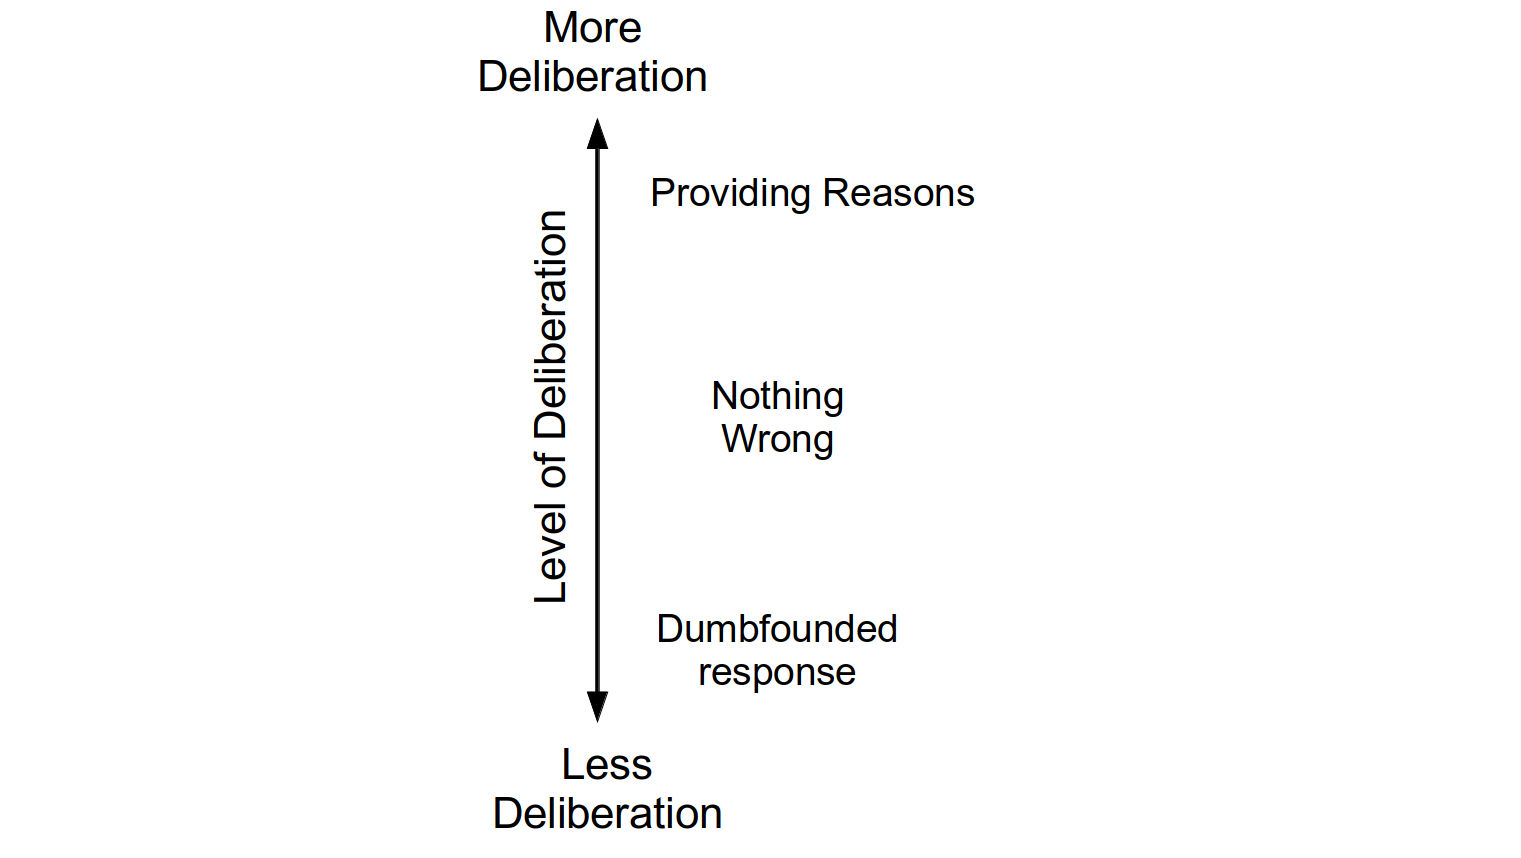
\includegraphics{../resources/images/responses_figure2.png}
\caption{hypothesized relationship between responses in the dumbfounding paradigm and level of deliberation}
\end{figure}

To understand moral dumbfounding as a conflict in dual-processes, we classified the responses in the dumbfounding paradigm as involving more or less deliberation. There are typically three responses in the dumbfounding paradigm: (1) the providing of reasons (reason); (2) accepting the counter-arguments and rating the behavior as \enquote{not wrong} (nothing wrong); or (3) a dumbfounded response (dumbfounding). Drawing on existing theorizing (e.g., Cushman, 2013; Haidt, 2001; McHugh et al., 2021) we hypothesize that making a judgment involves an intuitive/habitual response, involving relatively little deliberation, while providing reasons for judgment requires more deliberation (a deliberative response). We propose that dumbfounding occurs when the habitual response (the judgment) is in conflict with the deliberative response (providing reasons for the judgment). The dumbfounding paradigm additionally involves a third response, where participants may accept the counter-arguments and change their judgment, we hypothesize that this response involves more deliberation than a dumbfounded response but less deliberation than providing reasons. The hypothesized relative amounts of deliberation for each response are outlined in Figure 1.

\hypertarget{influences-on-moral-dumbfounding}{%
\section{Influences on Moral Dumbfounding}\label{influences-on-moral-dumbfounding}}

A core prediction of explaining dumbfounding as conflict in dual-processes is that under specific manipulations, responses in the moral dumbfounding paradigm should vary in predictable ways. Cognitive load has been shown to inhibit deliberative responding (e.g., De Neys, 2006; Evans \& Curtis-Holmes, 2005; Evans \& Stanovich, 2013; Schmidt, 2016). Above, we identified providing reasons as involving more deliberation than alternative responses in the dumbfounding paradigm. This implies that cognitive load should inhibit the identification of reasons for a judgment, leading to an increase in dumbfounded responding or an increase in accepting the counter-arguments and revising the judgment made.

\hypertarget{refs}{}
\leavevmode\hypertarget{ref-bago_intuitive_2019}{}%
Bago, B., \& De Neys, W. (2019). The intuitive greater good: Testing the corrective dual process model of moral cognition. \emph{Journal of Experimental Psychology: General}, \emph{148}(10), 1782--1801. \url{https://doi.org/10.1037/xge0000533}

\leavevmode\hypertarget{ref-bonner_conflict_2010}{}%
Bonner, C., \& Newell, B. R. (2010). In conflict with ourselves? An investigation of heuristic and analytic processes in decision making. \emph{Memory \& Cognition}, \emph{38}(2), 186--196. \url{https://doi.org/10.3758/MC.38.2.186}

\leavevmode\hypertarget{ref-brand_dualprocess_2016}{}%
Brand, C. (2016). \emph{Dual-Process Theories in Moral Psychology: Interdisciplinary Approaches to Theoretical, Empirical and Practical Considerations}. Springer. Retrieved from \url{http://books.google.com?id=nQ3NCwAAQBAJ}

\leavevmode\hypertarget{ref-crockett_models_2013}{}%
Crockett, M. J. (2013). Models of morality. \emph{Trends in Cognitive Sciences}, \emph{17}(8), 363--366. \url{https://doi.org/10.1016/j.tics.2013.06.005}

\leavevmode\hypertarget{ref-cushman_action_2013}{}%
Cushman, F. A. (2013). Action, Outcome, and Value A Dual-System Framework for Morality. \emph{Personality and Social Psychology Review}, \emph{17}(3), 273--292. \url{https://doi.org/10.1177/1088868313495594}

\leavevmode\hypertarget{ref-cushman_multisystem_2010}{}%
Cushman, F. A., Young, L., \& Greene, J. D. (2010). Multi-system Moral Psychology. In J. M. Doris (Ed.), \emph{The Moral Psychology Handbook} (pp. 47--71). Oxford; New York: Oxford University Press.

\leavevmode\hypertarget{ref-deneys_dual_2006}{}%
De Neys, W. (2006). Dual Processing in Reasoning: Two Systems but One Reasoner. \emph{Psychological Science}, \emph{17}(5), 428--433. \url{https://doi.org/10.1111/j.1467-9280.2006.01723.x}

\leavevmode\hypertarget{ref-deneys_bias_2012}{}%
De Neys, W. (2012). Bias and Conflict: A Case for Logical Intuitions. \emph{Perspectives on Psychological Science}, \emph{7}(1), 28--38. \url{https://doi.org/10.1177/1745691611429354}

\leavevmode\hypertarget{ref-deneys_conflict_2008}{}%
De Neys, W., \& Glumicic, T. (2008). Conflict monitoring in dual process theories of thinking. \emph{Cognition}, \emph{106}(3), 1248--1299. \url{https://doi.org/10.1016/j.cognition.2007.06.002}

\leavevmode\hypertarget{ref-deneys_logic_2019}{}%
De Neys, W., \& Pennycook, G. (2019). Logic, Fast and Slow: Advances in Dual-Process Theorizing. \emph{Current Directions in Psychological Science}, \emph{28}(5), 503--509. \url{https://doi.org/10.1177/0963721419855658}

\leavevmode\hypertarget{ref-evans_resolution_2007}{}%
Evans, J. S. B. T. (2007). On the resolution of conflict in dual process theories of reasoning. \emph{Thinking \& Reasoning}, \emph{13}(4), 321--339. \url{https://doi.org/10.1080/13546780601008825}

\leavevmode\hypertarget{ref-evans_rapid_2005}{}%
Evans, J. S. B. T., \& Curtis-Holmes, J. (2005). Rapid responding increases belief bias: Evidence for the dual-process theory of reasoning. \emph{Thinking \& Reasoning}, \emph{11}(4), 382--389. \url{https://doi.org/10.1080/13546780542000005}

\leavevmode\hypertarget{ref-evans_dualprocess_2013}{}%
Evans, J. S. B. T., \& Stanovich, K. E. (2013). Dual-Process Theories of Higher Cognition: Advancing the Debate. \emph{Perspectives on Psychological Science}, \emph{8}(3), 223--241. \url{https://doi.org/10.1177/1745691612460685}

\leavevmode\hypertarget{ref-greene_secret_2008}{}%
Greene, J. D. (2008). The Secret Joke of Kant's Soul. In W. Sinnott-Armstrong, \emph{Moral Psychology Volume 3: The neurosciences of morality: Emotion, brain disorders, and development} (pp. 35--79). Cambridge (Mass.): the MIT press.

\leavevmode\hypertarget{ref-guglielmo_unfounded_2018}{}%
Guglielmo, S. (2018). Unfounded dumbfounding: How harm and purity undermine evidence for moral dumbfounding. \emph{Cognition}, \emph{170}, 334--337. \url{https://doi.org/10.1016/j.cognition.2017.08.002}

\leavevmode\hypertarget{ref-haidt_emotional_2001}{}%
Haidt, J. (2001). The emotional dog and its rational tail: A social intuitionist approach to moral judgment. \emph{Psychological Review}, \emph{108}(4), 814--834. \url{https://doi.org/10.1037/0033-295X.108.4.814}

\leavevmode\hypertarget{ref-haidt_moral_2000}{}%
Haidt, J., Björklund, F., \& Murphy, S. (2000). Moral dumbfounding: When intuition finds no reason. \emph{Unpublished Manuscript, University of Virginia}.

\leavevmode\hypertarget{ref-lerner_when_1999}{}%
Lerner, M. J., \& Goldberg, J. H. (1999). When Do Decent People Blame Victims? The Differing Effects of the Explicit/Rational and Implicit/Experiential Cognitive Systems. In S. Chaiken \& Y. Trope (Eds.), \emph{Dual-process Theories in Social Psychology} (pp. 627--640). Guilford Press. Retrieved from \url{http://books.google.com?id=5X_auIBx99EC}

\leavevmode\hypertarget{ref-mchugh_searching_2017a}{}%
McHugh, C., McGann, M., Igou, E. R., \& Kinsella, E. L. (2017). Searching for Moral Dumbfounding: Identifying Measurable Indicators of Moral Dumbfounding. \emph{Collabra: Psychology}, \emph{3}(1), 1--24. \url{https://doi.org/10.1525/collabra.79}

\leavevmode\hypertarget{ref-mchugh_reasons_2020}{}%
McHugh, C., McGann, M., Igou, E. R., \& Kinsella, E. L. (2020). Reasons or rationalizations: The role of principles in the moral dumbfounding paradigm. \emph{Journal of Behavioral Decision Making}, \emph{33}(3), 376--392. \url{https://doi.org/10.1002/bdm.2167}

\leavevmode\hypertarget{ref-mchugh_moral_2021}{}%
McHugh, C., McGann, M., Igou, E. R., \& Kinsella, E. L. (2021). Moral Judgment as Categorization (MJAC). \emph{Perspectives on Psychological Science}. \url{https://doi.org/10.1177/1745691621990636}

\leavevmode\hypertarget{ref-prinz_passionate_2005}{}%
Prinz, J. J. (2005). Passionate Thoughts: The Emotional Embodiment of Moral Concepts. In D. Pecher \& R. A. Zwaan (Eds.), \emph{Grounding Cognition: The Role of Perception and Action in Memory, Language, and Thinking} (pp. 93--114). Cambridge University Press.

\leavevmode\hypertarget{ref-royzman_curious_2015}{}%
Royzman, E. B., Kim, K., \& Leeman, R. F. (2015). The curious tale of Julie and Mark: Unraveling the moral dumbfounding effect. \emph{Judgment and Decision Making}, \emph{10}(4), 296--313.

\leavevmode\hypertarget{ref-rozin_sensitivity_1994}{}%
Rozin, P., Markwith, M., \& McCauley, C. (1994). Sensitivity to indirect contacts with other persons: AIDS aversion as a composite of aversion to strangers, infection, moral taint, and misfortune. \emph{Journal of Abnormal Psychology}, \emph{103}(3), 495--504. \url{https://doi.org/10.1037/0021-843X.103.3.495}

\leavevmode\hypertarget{ref-schmidt_effects_2016}{}%
Schmidt, D. (2016). The Effects of Cognitive Load and Stereotyped Groups on Punitiveness. \emph{CMC Senior Theses}.

\leavevmode\hypertarget{ref-tversky_extensional_1983}{}%
Tversky, A., \& Kahneman, D. (1983). Extensional versus intuitive reasoning: The conjunction fallacy in probability judgment. \emph{Psychological Review}, \emph{90}(4), 293--315. \url{https://doi.org/10.1037/0033-295X.90.4.293}


\clearpage
\renewcommand{\listfigurename}{Figure captions}

\clearpage
\renewcommand{\listtablename}{Table captions}


\end{document}
